% !TeX program = pdfLaTeX
\documentclass[12pt]{article}
\usepackage{amsmath}
\usepackage{graphicx,psfrag,epsf}
\usepackage{enumerate}
\usepackage{natbib}
\usepackage{textcomp}
\usepackage[hyphens]{url} % not crucial - just used below for the URL
\usepackage{hyperref}
\providecommand{\tightlist}{%
  \setlength{\itemsep}{0pt}\setlength{\parskip}{0pt}}

%\pdfminorversion=4
% NOTE: To produce blinded version, replace "0" with "1" below.
\newcommand{\blind}{0}

% DON'T change margins - should be 1 inch all around.
\addtolength{\oddsidemargin}{-.5in}%
\addtolength{\evensidemargin}{-.5in}%
\addtolength{\textwidth}{1in}%
\addtolength{\textheight}{1.3in}%
\addtolength{\topmargin}{-.8in}%

%% load any required packages here



% Pandoc citation processing

\usepackage[dvipsnames]{xcolor} % colors
\newcommand{\ear}[1]{{\textcolor{blue}{#1}}}
\newcommand{\svp}[1]{{\textcolor{RedOrange}{#1}}}
\newcommand{\rh}[1]{{\textcolor{Green}{#1}}}
\usepackage[capitalise]{cleveref}
\newcommand\pcref[1]{(\cref{#1})}
\usepackage{algorithm,algpseudocode,booktabs}

\begin{document}


\def\spacingset#1{\renewcommand{\baselinestretch}%
{#1}\small\normalsize} \spacingset{1}


%%%%%%%%%%%%%%%%%%%%%%%%%%%%%%%%%%%%%%%%%%%%%%%%%%%%%%%%%%%%%%%%%%%%%%%%%%%%%%

\if0\blind
{
  \title{\bf Eye Fitting Straight Lines in the Modern Era}

  \author{
        Emily A. Robinson 1 \\
    Department of Statistics, University of Nebraska - Lincoln\\
     and \\     Susan VanderPlas 2 \\
    Department of Statistics, University of Nebraska - Lincoln\\
     and \\     Reka Howard 3 \\
    Department of Statistics, University of Nebraska - Lincoln\\
      }
  \maketitle
} \fi

\if1\blind
{
  \bigskip
  \bigskip
  \bigskip
  \begin{center}
    {\LARGE\bf Eye Fitting Straight Lines in the Modern Era}
  \end{center}
  \medskip
} \fi

\bigskip
\begin{abstract}
Fitting lines by eye through a set of points has been explored since the
20th century. Common methods of fitting trends by eye involve
maneuvering a string, black thread, or ruler until the fit is suitable,
then drawing the line through the set of points. In 2015, the New York
Times introduced an interactive feature, called `You Draw It'. Readers
are asked to input their own assumptions about various metrics and
compare how these assumptions relate to reality. The New York Times team
utilizes Data Driven Documents (D3) that allows readers to predict these
metrics by drawing a line on their computer screen with their computer
mouse. In my research, I established `You Draw It' as a method for
graphical testing by adapting the New York Times feature. I recruited
participants via crowdsourcing websites and replicated the study found
in Eye Fitting Straight Lines (Mosteller et al., 1981). Participants
were directed to an RShiny application link and shown points following a
linear trend and asked to draw a line through the data points using
their computer mouse; task plots were generated using the r2d3 package
in R statistical software. Results from my study were consistent with
those found in the previous study; when shown points following a linear
trend, participants tended to fit the slope of the first principal
component over the slope of the least-squares regression line. This
trend was most prominent when shown data simulated with larger
variances. The reproducibility of these results serves as evidence of
the reliability of the you draw it method. Future work is necessary to
implement the `You Draw It' tool as a method of testing graphics. {[}200
word limit{]}
\end{abstract}

\noindent%
{\it Keywords:} Graphics, Regression, Graph
Perception, Scatterplot, Cognitive Bias
\vfill

\newpage
\spacingset{1.45} % DON'T change the spacing!

\hypertarget{introduction}{%
\section{Introduction}\label{introduction}}

\begin{itemize}
\tightlist
\item
  What are graphs? Why do we care?
\end{itemize}

\hypertarget{graph-perception}{%
\subsection{Graph Perception}\label{graph-perception}}

\begin{itemize}
\tightlist
\item
  Cleveland and McGill
\end{itemize}

\hypertarget{testing-statistical-graphics}{%
\subsection{Testing Statistical
Graphics}\label{testing-statistical-graphics}}

Graphical tests are useful for studying the perception of statistical
graphs. Studies might ask participants to identify differences in
graphs, read information off of a chart accurately, use data to make
correct real-world decisions, or predict the next few observations. All
of these types of tests require different levels of use and manipulation
of the information being presented in the chart. Early researchers
studied graphs from a psychological perspective. These studies generally
tested participants ability to detect a stimulus (or a difference
between two stimuli) ({\textcolor{blue}{CITATIONS}}). Here we focus on
the how graphical testing has developed in statistics.

A major development in statistical graphics research is Wilkinson's
Grammar of Graphics \citep{wilkinson2013grammar}. The grammar of
graphics serves as the fundamental framework for data visualization with
the notion that graphics are built from the ground up by specifying
exactly how to create a particular graph from a given data set. Visual
representations are constructed through the use of ``tidy data'' which
is characterized as a data set in which each variable is in its own
column, each observation is in its own row, and each value is in its own
cell \citep{wickham2016r}. Graphics are viewed as a mapping from
variables in a data set (or statistics computed from the data) to visual
attributes such as the axes, colors, shapes, or facets on the canvas in
which the chart is displayed. Software, such as Hadley Wickham's ggplot2
\citep{wickham2011ggplot2}, aims to implement the framework of creating
charts and graphics as the grammar of graphics recommends.

One useful tool for testing statistical graphics is the concept of a
lineup. \citet{buja2009statistical} introduced the lineup protocol in
which data plots are depicted and interpreted as statistics. Supported
by the grammar of graphics, a data plot can be characterized as a
statistic, defined as, ``a functional mapping of a variable or set of
variables'' \citep{vanderplas2020testing}. This allows the data plot to
be tested similar to other statistics, by comparing the actual data plot
to a set of plots with the absence of any data structure we can test the
likelihood of any perceived structure being significant. The
construction of data plots as statistics allow for easy experimentation,
granting researchers the ability to compare the effectiveness of and
understand the perception of different types of charts
({\textcolor{blue}{CITATIONS}}). The lineup protocol is one such example
of the development of tools designed for statistical graphical testing.
The advancement of graphing software provides the tools necessary to
develop new methods of testing graphics.

\hypertarget{fitting-trends-by-eye}{%
\subsection{Fitting Trends by Eye}\label{fitting-trends-by-eye}}

Initial studies in the 20th century explored the use of fitting lines by
eye through a set of points
\citep{finney1951subjective, mosteller1981eye}. Common methods of
fitting trends by eye involved maneuvering a string, black thread, or
ruler until the fit is suitable, then drawing the line through the set
of points. Recently, \citet{ciccione2021can} conducted a comprehensive
set of studies investigating human ability to detect trends in graphical
representations from a psychophysical approach.

In \citet{finney1951subjective}, it was of interest to determine the
effect of stopping iterative maximum likelihood calculations after one
iteration. Many techniques in statistical analysis are performed with
the aid of iterative calculations such as Newton's method or Fisher's
scoring. The author was interested in whether one iteration of
calculations was sufficient in the estimation of parameters connected
with dose-response relationships. One measure of interest is the
relative potency between a test preparation of doses and standard
preparation of does; relative potency is calculated as the ratio of two
equally effective doses between the two preparation methods. In this
study, twenty-one scientists were recruited via postal mail and asked to
``rule two lines'' in order to judge by eye the positions for a pair of
parallel probit regression lines in a biological assay. The author then
computed one iterative calculation of the relative potency based on
starting values as indicated by the pair of lines provided by each
participant and compared these relative potency estimates to that which
was estimated by the full probit technique (reaching convergence through
multiple iterations). Results indicated that one cycle of iterations for
calculating the relative potency was sufficient based on the starting
values provided by eye from the participants.

\citet{mosteller1981eye}, sought to understand the properties of least
squares and other computed lines by establishing one systematic method
of fitting lines by eye. Participants were asked to fit lines by eye to
four scatter-plots using an 8.5 x 11 inch transparency with a straight
line etched completely across the middle. A latin square design with
packets of the set of points stapled together in four different
sequences was used to determine if there is an effect of order of
presentation. It was found that order of presentation had no effect and
that participants tended to fit the slope of the principal axis (error
minimized orthogonally, both horizontal and vertical, to the regression
line) over the slope of the least squares regression line (error
minimized vertically to the regression line). These results support
previous research on ``ensemble perception'' indicating the visual
system can compute averages of various features in parallel across the
items in a set ({\textcolor{blue}{CITATIONS}}).

In \citet{ciccione2021can}, participants were asked to judge trends,
estimate slopes, and conduct extrapolation. To estimate slopes,
participants were asked to report the slope of the best-fitting
regression line using a trackpad to adjust the tilt of a line on screen.
Results indicated the slopes participants reported were always in excess
of the ideal slopes, both in the positive and in the negative direction,
and those biases increase with noise and with number of points. This
supports the results found in \citet{mosteller1981eye} and suggest that
participants might use Deming regression when fitting a line to a noisy
scatterplot.

In 2015, the New York Times introduced an interactive feature, called
You Draw It
\citep{aisch_cox_quealy_2015, buchanan_park_pearce_2017, katz_2017}.
Readers are asked to input their own assumptions about various metrics
and compare how these assumptions relate to reality. The New York Times
team utilizes Data Driven Documents (D3) that allows readers to predict
these metrics through the use of drawing a line on their computer screen
with their computer mouse. After the reader has completed drawing the
line, the actual observed values are revealed and the reader may check
their estimated knowledge against the actual reported data.

\hypertarget{research-objectives}{%
\subsection{Research objectives}\label{research-objectives}}

In this paper, we establish `You Draw It', adapted from the New York
Times feature, as tool for graphical testing. The `You Draw It' method
is validated by replicating the study conducted by
\citet{mosteller1981eye}. The results of our study provide support for
``ensemble perception''.

\hypertarget{methods}{%
\section{Methods}\label{methods}}

\hypertarget{participants}{%
\subsection{Participants}\label{participants}}

Participants were recruited through through Twitter, Reddit, and direct
email in May 2021. A total of 39 individuals completed 256 unique `You
Draw It' task plots; all completed you draw it task plots were included
in the analysis. All participants had normal or corrected to normal
vision and signed an informed consent form. The experimental tasks took
approximately 15 minutes to complete. Participants completed the
experiment on their own computers in an environment of their choosing.
The experiment was conducted and distributed through an RShiny
application found
\href{https://shiny.srvanderplas.com/you-draw-it/}{here}.

\hypertarget{you-draw-it-task}{%
\subsection{`You Draw It' Task}\label{you-draw-it-task}}

Data Driven Documents (D3), a JavaScript-based graphing framework that
facilitates user interaction, is used to create the `You Draw It' task
plots. Integrating this into RShiny using the r2d3 package, participants
are asked to draw a line using their computer mouse through trend shown
on their screen. Details of the development of the `You Draw It' task
plots will be addressed in future work. In the study, participants are
shown an interactive scatter-plot \cref{fig:ydi-stimuli} along with the
prompt, ``Use your mouse to fill in the trend in the yellow box
region.'' The yellow-box region moves along as the participant draws
their trend-line until the yellow region disappears, indicating the
participant has filled in the entire domain.

\begin{figure}[tbp]

{\centering 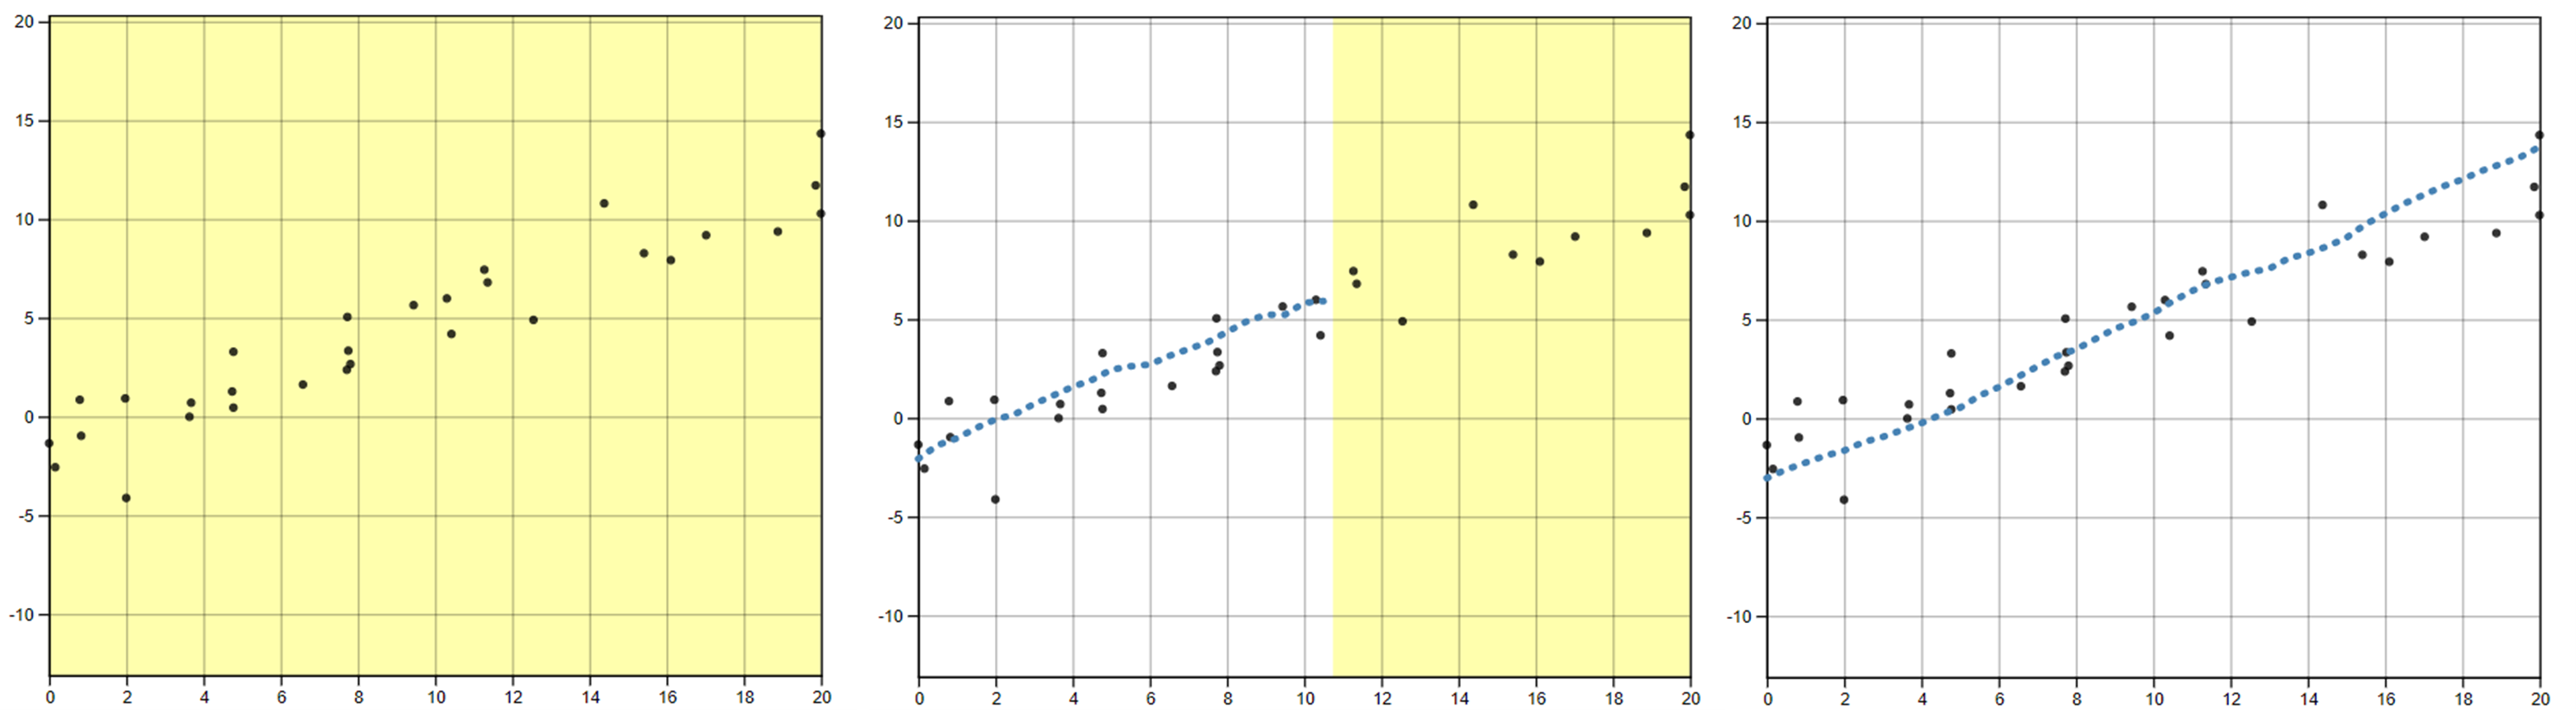
\includegraphics[width=1\linewidth,]{images/ydi-stimuli} 

}

\caption{'You Draw It' Stimuli}\label{fig:ydi-stimuli}
\end{figure}

\hypertarget{data-generation}{%
\subsection{Data Generation}\label{data-generation}}

All data processing was conducted in R statistical software. A total of
\(N = 30\) points \((x_i, y_i), i = 1,...N\) were generated for
\(x_i \in [x_{min}, x_{max}]\) where \(x\) and \(y\) have a linear
relationship. Data were simulated based on linear model with additive
errors: \begin{align}
y_i & = \beta_0 + \beta_1 x_i + e_i \\
\text{with } e_i & \sim N(0, \sigma^2). \nonumber
\end{align} The parameters \(\beta_0\) and \(\beta_1\) are selected to
replicate \citet{mosteller1981eye} with \(e_i\) generated by rejection
sampling in order to guarantee the points shown align with that of the
fitted line.

Simulated model equation parameters were selected to reflect the four
data sets (F, N, S, and V) used in \citet{mosteller1981eye}
(\cref{tab:eyefitting-parameters}). Parameter choices F, N, and S
simulated data across a domain of 0 to 20. Parameter choice F produces a
trend with a positive slope and a large variance while N has a negative
slope and a large variance. In comparison, S shows a trend with a
positive slope with a small variance and V yields a steep positive slope
with a small variance over the domain of 4 to 16.
\cref{fig:eyefitting-simplot} illustrates an example of simulated data
for all four parameter choices intended to reflect the trends in
\citet{mosteller1981eye}. Aesthetic design choices were made consistent
across each of the interactive you draw it plots. The y-axis range
extended 10\% beyond (above and below) the range of the simulated data
points to allow for users to draw outside the simulated data set range.

\begin{table}

\caption{\label{tab:eyefitting-parameters}Eye Fitting Straight Lines in the Modern Era simulation model parameters}
\centering
\begin{tabular}[t]{cccc}
\toprule
Parameter Choice & $y_{\bar{x}}$ & $\beta_1$ & $\sigma$\\
\midrule
S & 3.88 & 0.66 & 1.30\\
F & 3.90 & 0.66 & 1.98\\
V & 3.89 & 1.98 & 1.50\\
N & 4.11 & -0.70 & 2.50\\
\bottomrule
\end{tabular}
\end{table}

\begin{figure}[tbp]

{\centering 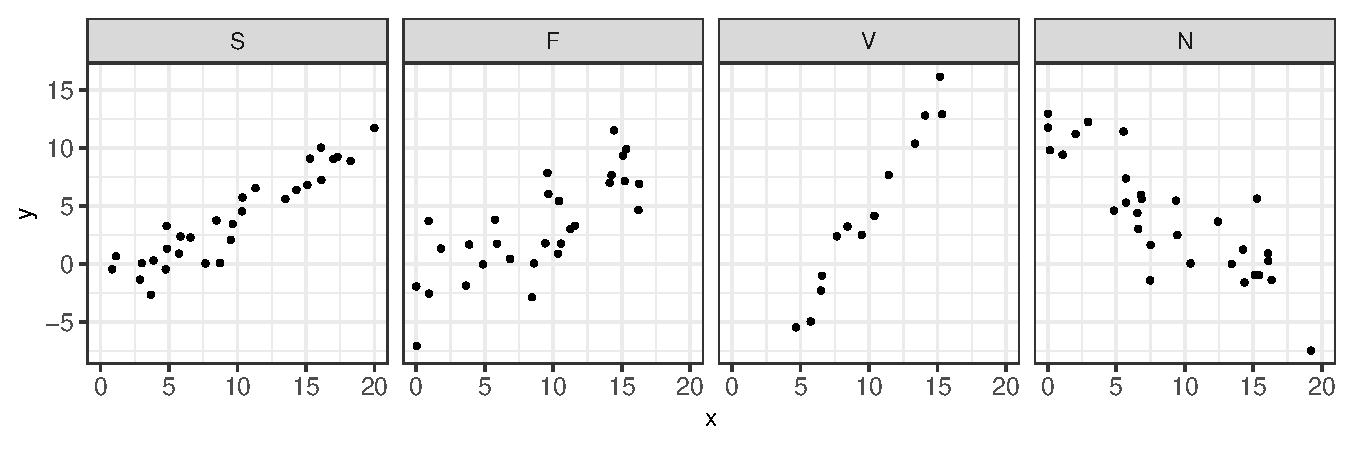
\includegraphics[width=1\linewidth,]{Eye-Fitting-Stright-Lines-in-the-Modern-Era_files/figure-latex/eyefitting-simplot-1} 

}

\caption{Eye Fitting Straight Lines in the Modern Era Simulated Data Example}\label{fig:eyefitting-simplot}
\end{figure}

\hypertarget{study-design}{%
\subsection{Study Design}\label{study-design}}

This experiment was conducted as part of a larger study; for simplicity,
we focus on the study design and methods related to the current study.
Each scatter-plot was the graphical representation of a data set that
was generated randomly, independently for each participant at the start
of the experiment. Participants in the study are shown two `You Draw It'
practice plots in order to train participants in the skills associated
with executing the task followed by four task plots associated with the
current study. The order of the task plots was randomly assigned for
each individual in a completely randomized design.

\hypertarget{results}{%
\section{Results}\label{results}}

\hypertarget{fitted-values}{%
\subsection{Fitted Values}\label{fitted-values}}

In addition to the participant drawn points, \((x_k, y_{k,drawn})\), and
the ordinary least squares (OLS) regression fitted values,
\((x_k, \hat y_{k,OLS})\), a regression equation with a slope based on
the first principal component (PCA) was used to calculate fitted values,
\((x_k, \hat y_{k,PCA})\). For each set of simulated data and parameter
choice, the PCA regression equation was determined by using the princomp
function in the stats package in base R to obtain the rotation of the
coordinate axes from the first principal component (direction which
captures the most variance). The estimated slope, \(\hat\beta_{1,PCA}\),
is determined by the ratio of the axis rotation in y and axis rotation
in x of the first principal component with the y-intercept,
\(\hat\beta_{0,PCA}\) calculated by the point-slope equation of a line
using the mean of of the simulated points, \((\bar x_i, \bar y_i)\).
Fitted values, \(\hat y_{k,PCA}\) are then obtained every 0.25 increment
across the domain from the PCA regression equation,
\(\hat y_{k,PCA} = \hat\beta_{0,PCA} + \hat\beta_{1,PCA} x_k\).
\cref{fig:ols-vs-pca-example} illustrates the difference between an OLS
regression equation which minimizes the vertical distance of points from
the line and a regression equation with a slope calculated by the first
principal component which minimizes the smallest distance of points from
the line.

\begin{itemize}
\tightlist
\item
  Because of the randomness in the stimulus generation process, on any
  given trial the actual slope of the linear regression line could
  differ from its prescribed value.
\end{itemize}

\hypertarget{feedback-data}{%
\subsection{Feedback Data}\label{feedback-data}}

\hypertarget{linear-trend-constraint-performance}{%
\subsection{Linear Trend Constraint
Performance}\label{linear-trend-constraint-performance}}

\hypertarget{smoothing-spline-trend-performance}{%
\subsection{Smoothing Spline Trend
Performance}\label{smoothing-spline-trend-performance}}

\hypertarget{discussion-and-conclusion}{%
\section{Discussion and Conclusion}\label{discussion-and-conclusion}}

\hypertarget{future-work}{%
\section{Future Work}\label{future-work}}

\begin{itemize}
\tightlist
\item
  Use the method.
\item
  Write R package.
\end{itemize}

\bibliographystyle{agsm}
\bibliography{bibliography.bib}

\end{document}
